\documentclass[journal]{IEEEtran}

\usepackage{amsmath,amsfonts,amssymb}
\usepackage{algorithmic}
\usepackage{algorithm}
\usepackage{array}
\usepackage{booktabs}
\usepackage{cite}
\usepackage{graphicx}
\usepackage{textcomp}
\usepackage{url}
\usepackage{xcolor}
\usepackage{hyperref}

\graphicspath{{./}{figures/}{../results/figures/}}
% ==============================================================================
% Canonical Experimental Numbers for Project Triathlon
% Single Source of Truth generated from results/
% ==============================================================================

% Primary Model (Multinomial Logistic Regression, 15 evaluations across 5 folds and 3 seeds)
\newcommand{\lrTopOneAcc}{58.4\%}
\newcommand{\lrTopOneStd}{6.9\%}
\newcommand{\lrMeanRegret}{1.56}
\newcommand{\lrMeanRegretStd}{0.31}
\newcommand{\lrMaxRegret}{13.1}

% Random Forest Comparator
\newcommand{\rfTopOneAcc}{52.6\%}
\newcommand{\rfTopOneStd}{6.0\%}
\newcommand{\rfMeanRegret}{2.06}
\newcommand{\rfMeanRegretStd}{0.41}
\newcommand{\rfMaxRegret}{13.4}

% HistGradientBoosting Comparator
\newcommand{\hgbTopOneAcc}{47.9\%}
\newcommand{\hgbTopOneStd}{5.3\%}
\newcommand{\hgbMeanRegret}{2.49}
\newcommand{\hgbMeanRegretStd}{0.45}
\newcommand{\hgbMaxRegret}{13.9}

% Baselines
\newcommand{\retinexRegret}{2.73}
\newcommand{\randomRegret}{7.03}
\newcommand{\oracleRegret}{0.00}

% Headroom & Dividends
\newcommand{\gainVsRetinex}{1.17}
\newcommand{\gainVsRandom}{5.47}
\newcommand{\oracleGapCaptured}{42.8\%}
\newcommand{\lrModelSize}{2.4\text{ KB}}
\newcommand{\rfModelSize}{3.5\text{ MB}}
\newcommand{\sizeRatio}{\ensuremath{\approx 1,493\times}}
\newcommand{\lrLatency}{\ensuremath{0.90\text{ ms} \pm 0.56\text{ ms}}}
\newcommand{\rfLatency}{\ensuremath{\text{N/A (unmatched)}}}
% \newcommand{\speedRatio}{\ensuremath{5\times}}
\newcommand{\featExtLatency}{\ensuremath{14.22\text{ ms} \pm 2.42\text{ ms}}}

% Zero-Shot Cross-Dataset (LOL-v2)
\newcommand{\lolvTwoRealRegret}{1.70}
\newcommand{\lolvTwoRealAcc}{36.0\%}
\newcommand{\lolvTwoRealRetinexRegret}{2.90}
\newcommand{\lolvTwoRealGain}{1.20}

\newcommand{\lolvTwoSynRegret}{3.44}
\newcommand{\lolvTwoSynAcc}{34.0\%}
\newcommand{\lolvTwoSynRetinexRegret}{3.60}
\newcommand{\lolvTwoSynGain}{0.16}


\begin{document}

\title{Fidelity-Driven Algorithm Selection for Low-Light Image Enhancement via Handcrafted Physical Statistics}

\author{Logi~Vasan,
        Suyash~Srivastav,
        Ananya~Kasaudhan,
        and~Kishor~P.~Upla,~\IEEEmembership{Senior~Member,~IEEE}%
\thanks{L. Vasan, S. Srivastav, and A. Kasaudhan are with the Department of Artificial Intelligence and Machine Learning, Gati Shakti Vishwavidyalaya, Vadodara 390004, Gujarat, India (e-mail: logivasan.aiml22@gsv.ac.in, suyashsri30@gmail.com).}%
\thanks{K. P. Upla is with the Department of Electronics Engineering, Sardar Vallabhbhai National Institute of Technology (SVNIT), Surat 395007, Gujarat, India (e-mail: kpu@eed.svnit.ac.in).}%
}

\markboth{IEEE Transactions on Image Processing (Under Review)}%
{Vasan \MakeLowercase{\textit{et al.}}: Fidelity-Driven Algorithm Selection for Low-Light Image Enhancement}

\maketitle

\begin{abstract}
Image enhancement is an ill-posed inverse problem where underexposure and photon noise destroy scene irradiance. While numerous enhancement operators exist, no single method dominates across all real-world scenes. Deployed edge systems routinely apply a static operator because full-reference fidelity metrics (PSNR, SSIM) are unavailable at inference time, while standard no-reference quality assessment (NR-IQA) metrics can fail catastrophically at fidelity ranking (achieving 0\% top-1 accuracy in recent low-light benchmarks). We formulate enhancement selection through decision theory under classical machine learning and CPU-only operational constraints. We propose a reference-free selector extracting an 8-dimensional physical descriptor vector spanning exposure, contrast, entropy, sensor noise, dark channel transmission, edge gradient distributions, and colourfulness in $\featExtLatency$ on CPU exclusively from the degraded input. Using an offline oracle constructed with full-reference fidelity supervision on the Low-Light (LOL-v1) benchmark, we train classical learners under strict 5-fold grouped cross-validation by scene across three seeds (15 evaluations). Our primary Multinomial Logistic Regression selector achieves $\mathbf{\lrTopOneAcc \pm \lrTopOneStd}$ accuracy and slashes mean decision regret to $\mathbf{\lrMeanRegret \pm \lrMeanRegretStd\text{ dB}}$, outperforming the best-fixed Retinex baseline ($\retinexRegret\text{ dB}$) by $\mathbf{\gainVsRetinex\text{ dB}}$ and capturing $\mathbf{\oracleGapCaptured}$ of the oracle gap. Under Occam's razor, Logistic Regression decisively outperforms Random Forest ($\rfMeanRegret\text{ dB}$) and HistGradientBoosting ($\hgbMeanRegret\text{ dB}$) while requiring $\sizeRatio$ less memory ($\lrModelSize$) with sub-millisecond CPU inference ($\lrLatency$). Zero-shot validation on LOL-v2 confirms positive transfer on real camera hardware ($\lolvTwoRealRegret\text{ dB}$ regret vs. $\lolvTwoRealRetinexRegret\text{ dB}$ for Retinex), while revealing synthetic domain shift limitations.
\end{abstract}

\begin{IEEEkeywords}
Algorithm selection, low-light image enhancement, decision regret, handcrafted physical features, classical machine learning, edge computing, Retinex, GroupKFold cross-validation.
\end{IEEEkeywords}

\section{Introduction}
\IEEEPARstart{D}{igital} imaging under photon-starved conditions—such as nighttime surveillance, intelligent transportation, and mobile photography—suffers from severe loss of contrast, non-uniform underexposure, and sensor grain \cite{zheng2024lowlight, wei2018deep}. An observed degraded frame $g(x)$ is governed by:
\begin{equation}
g(x) = \mathcal{H}[f(x)] + n(x),
\label{eq:degradation_model}
\end{equation}
where $f(x)$ is true scene radiance, $\mathcal{H}$ represents optical and exposure attenuation, and $n(x)$ is sensor noise \cite{chen2018learning}. Because forward attenuation irreversibly collapses dynamic range, inverting \eqref{eq:degradation_model} is severely ill-posed: multiple distinct scenes map onto identical degraded measurements.

Four decades of research have produced diverse enhancement families \cite{zheng2024lowlight}: point-wise gamma remapping, adaptive histogram equalization (CLAHE) \cite{zuiderveld1994contrast}, Retinex decomposition \cite{land1971lightness, jobson1997multiscale}, edge-preserving filtering \cite{tomasi1998bilateral}, and deep neural estimators \cite{wei2018deep, guo2020zero}. Practical deployments, however, face a fundamental challenge: \textit{no single enhancement operator dominates across all instances} \cite{wolpert1997no}. Retinex excels at non-uniform illumination but amplifies noise on photon-starved frames; histogram equalization maximizes contrast in flat scenes but causes unnatural saturation elsewhere. 

Full-reference metrics (PSNR, SSIM) \cite{wang2004image, hore2010image} cannot be computed at inference time because clean ground truth $f(x)$ is absent. Systems are thus forced to apply a static ``best average'' operator to every frame, incurring steep fidelity penalties. Crucially, recent empirical benchmarks (e.g., Lyu \textit{et al.}, BlindPSNR, 2026 \cite{lyu2026blindpsnr}) report that standard No-Reference IQA metrics (such as BRISQUE \cite{mittal2012no} and NIQE \cite{mittal2013making}) can fail severely at fidelity ranking, achieving 0\% top-1 accuracy on low-light enhancement selection because they reward synthetic sharpness and smoothing over fidelity to true scene radiance. If broadly reproducible, this motivates reference-free selection grounded directly in observable physical degradation statistics.

To overcome this dilemma without heavy deep networks, we investigate:
\noindent\textit{\textbf{Research Question (RQ1):} Can lightweight physical degradation statistics extracted strictly from degraded inputs reliably predict the PSNR-optimal enhancer, beating static baselines in accuracy and decision regret on unseen scenes?}

We formulate enhancement selection through John Rice's \textit{algorithm selection problem} \cite{rice1976algorithm}. By extracting an 8-dimensional descriptor vector $\phi(x)$ spanning seven physical degradation categories in $\featExtLatency$ on CPU, we train classical learners against an offline full-reference oracle under strict operational constraints: classical ML only, CPU-only execution, public benchmarks, and fixed enhancement portfolios.

\noindent\textbf{Key Contributions:}
\begin{itemize}
    \setlength{\itemsep}{1pt}
    \setlength{\parskip}{0pt}
    \item \textbf{Decision-Theoretic Regret Formulation}: We establish a selection framework pairing top-1 accuracy with non-negative decibel decision regret $\mathcal{R}(x) = \text{PSNR}_{\text{oracle}}(x) - \text{PSNR}_{\text{pred}}(x) \ge 0\text{ dB}$, heavily penalizing severe quality collapses while treating near-ties tolerantly.
    \item \textbf{Lightweight Handcrafted Descriptors}: We design an 8-D physical feature vector computed directly on degraded inputs in $\featExtLatency$ on CPU, completely bypassing candidate filter execution.
    \item \textbf{Leakage-Free Grouped Benchmark}: Under 5-fold \texttt{GroupKFold} by scene across 3 seeds (15 evaluations) on LOL-v1, our Multinomial Logistic Regression selector achieves $\mathbf{\lrTopOneAcc \pm \lrTopOneStd}$ accuracy and slashes mean regret to $\mathbf{\lrMeanRegret \pm \lrMeanRegretStd\text{ dB}}$, outperforming Best-Fixed Retinex ($\retinexRegret\text{ dB}$) by $\mathbf{\gainVsRetinex\text{ dB}}$ and capturing $\mathbf{\oracleGapCaptured}$ of available oracle headroom.
    \item \textbf{Occam's Razor Model Parsimony}: We resolve the linear versus ensemble debate: regularized Logistic Regression decisively outperforms Random Forest ($\rfMeanRegret\text{ dB}$) and HistGradientBoosting ($\hgbMeanRegret\text{ dB}$), while requiring $\sizeRatio$ less storage ($\lrModelSize$) and executing in $\lrLatency$ on CPU.
    \item \textbf{External Validation on LOL-v2}: Zero-shot evaluation on LOL-v2 without retraining demonstrates positive transfer on real camera hardware ($\lolvTwoRealRegret\text{ dB}$ regret vs. $\lolvTwoRealRetinexRegret\text{ dB}$ for Retinex), while characterizing synthetic Poisson noise shift limitations.
\end{itemize}

\section{Problem Formulation \& Decision Theory}

\subsection{Mathematical Setup and Oracle Selection}
Let $\mathcal{X}$ denote the degraded image domain, and let $\mathcal{A} = \{a_1, \dots, a_K\}$ represent a fixed bank of $K=6$ enhancement operators. For any input $x \in \mathcal{X}$, candidate output is $\hat{y}_a = a(x)$. When clean reference $y \in \mathcal{Y}$ is available offline, enhancement quality is quantified by full-reference fidelity $s_a(x) \triangleq \text{PSNR}(\hat{y}_a, y)$ in dB.

The \textbf{Oracle Selector} $a^*(x)$ is defined as the algorithm maximizing fidelity on instance $x$:
\begin{equation}
a^*(x) \triangleq \arg\max_{a \in \mathcal{A}} s_a(x).
\label{eq:oracle_definition}
\end{equation}
A deployed selector $\pi: \mathcal{X} \to \mathcal{A}$ maps observable features $\phi(x) \in \mathbb{R}^8$ extracted from degraded input $x$ directly to an operator choice, without access to $y$ or forward candidate outputs.

\subsection{Decision Regret Formulation}
Classification accuracy alone is an inadequate objective for algorithm selection \cite{bischl2016aslib}: misclassifying between two near-tied operators ($30.02\text{ dB}$ vs. $30.00\text{ dB}$) incurs an imperceptible $0.02\text{ dB}$ loss, whereas choosing an inappropriate operator that posterizes edges may cost $10\text{ dB}$. We formally quantify performance via \textbf{Decision Regret}:
\begin{equation}
\mathcal{R}(x, \pi) \triangleq s_{a^*}(x) - s_{\pi(x)}(x) \ge 0\text{ dB}.
\label{eq:regret_definition}
\end{equation}
Across an evaluation corpus of $N$ instances, we evaluate mean regret $\bar{\mathcal{R}}(\pi) = \frac{1}{N} \sum_{i=1}^N \mathcal{R}(x_i, \pi)$ and maximum regret $\mathcal{R}_{\max}(\pi) = \max_i \mathcal{R}(x_i, \pi)$. The objective is minimizing expected regret $\mathbb{E}[\mathcal{R}(x, \pi)]$ over the target distribution.

\subsection{Leakage-Free Experimental Protocol}
To ensure rigorous generalization estimates, we enforce three strict boundaries:
\begin{enumerate}
    \setlength{\itemsep}{1pt}
    \setlength{\parskip}{0pt}
    \item \textbf{Scene Grouping (\texttt{GroupKFold})}: Partitioning is strictly grouped by 64-bit reference dHash connected components (Hamming distance $\le 10$, 228 disjoint scene clusters). All multi-exposure photographic variants of a scene remain strictly isolated within train or validation folds.
    \item \textbf{Preprocessing Isolation}: Feature standardization parameters ($\mu_{\text{tr}}, \sigma_{\text{tr}}$) are fitted strictly within training folds inside encapsulated pipelines (\texttt{make\_pipeline(StandardScaler(), model)}).
    \item \textbf{Label Isolation}: Feature extractor $\phi(x)$ ingests degraded image $g(x)$ only. Ground truth is accessed exclusively to populate the offline score matrix.
\end{enumerate}

\section{Lightweight Physical Descriptors \& Portfolio}

\subsection{The Six-Method Enhancement Bank (\texorpdfstring{$\mathcal{A}$}{A})}
We establish a six-operator portfolio with complementary inductive biases:
\begin{enumerate}
    \setlength{\itemsep}{1pt}
    \setlength{\parskip}{0pt}
    \item \textbf{Identity ($a_1$)}: $\hat{y}=x$. The essential do-nothing baseline for well-exposed frames.
    \item \textbf{Gamma Correction ($a_2$)}: Monotonic shadow expansion via 256-entry lookup table $s = 255 \cdot (r/255)^{0.5}$ ($\gamma=0.5$).
    \item \textbf{CLAHE ($a_3$)}: Contrast Limited Adaptive Histogram Equalization on CIELAB luminance ($\text{clipLimit}=2.0, 8\times 8$ grid) \cite{zuiderveld1994contrast}.
    \item \textbf{Histogram Equalization ($a_4$)}: Global cumulative distribution function (CDF) luminance remapping maximizing tonal spread over $[0, 255]$.
    \item \textbf{Single-Scale Retinex ($a_5$)}: Illumination estimation $\log R = \log I - \log (G_\sigma * I)$ with Gaussian surround $\sigma=80.0$ and dynamic normalization \cite{jobson1997multiscale}.
    \item \textbf{Bilateral Filtering + Unsharp Masking ($a_6$)}: Edge-preserving smoothing ($d=9, \sigma=75$) followed by unsharp masking ($\sigma=1.5, \alpha=0.8$) \cite{tomasi1998bilateral}.
\end{enumerate}
\noindent\textit{Portfolio Boundaries}: While inverted dark channel dehazing \cite{dong2011fast} is a known heuristic, low-light degradation is physically governed by Poisson shot noise rather than particulate scattering. Inverting dark channel noise induces chromatic distortion and requires $80$--$250\text{ ms}$ on CPU (violating real-time budgets); it is thus excluded from our real-time portfolio.

\begin{figure}[!t]
\centering
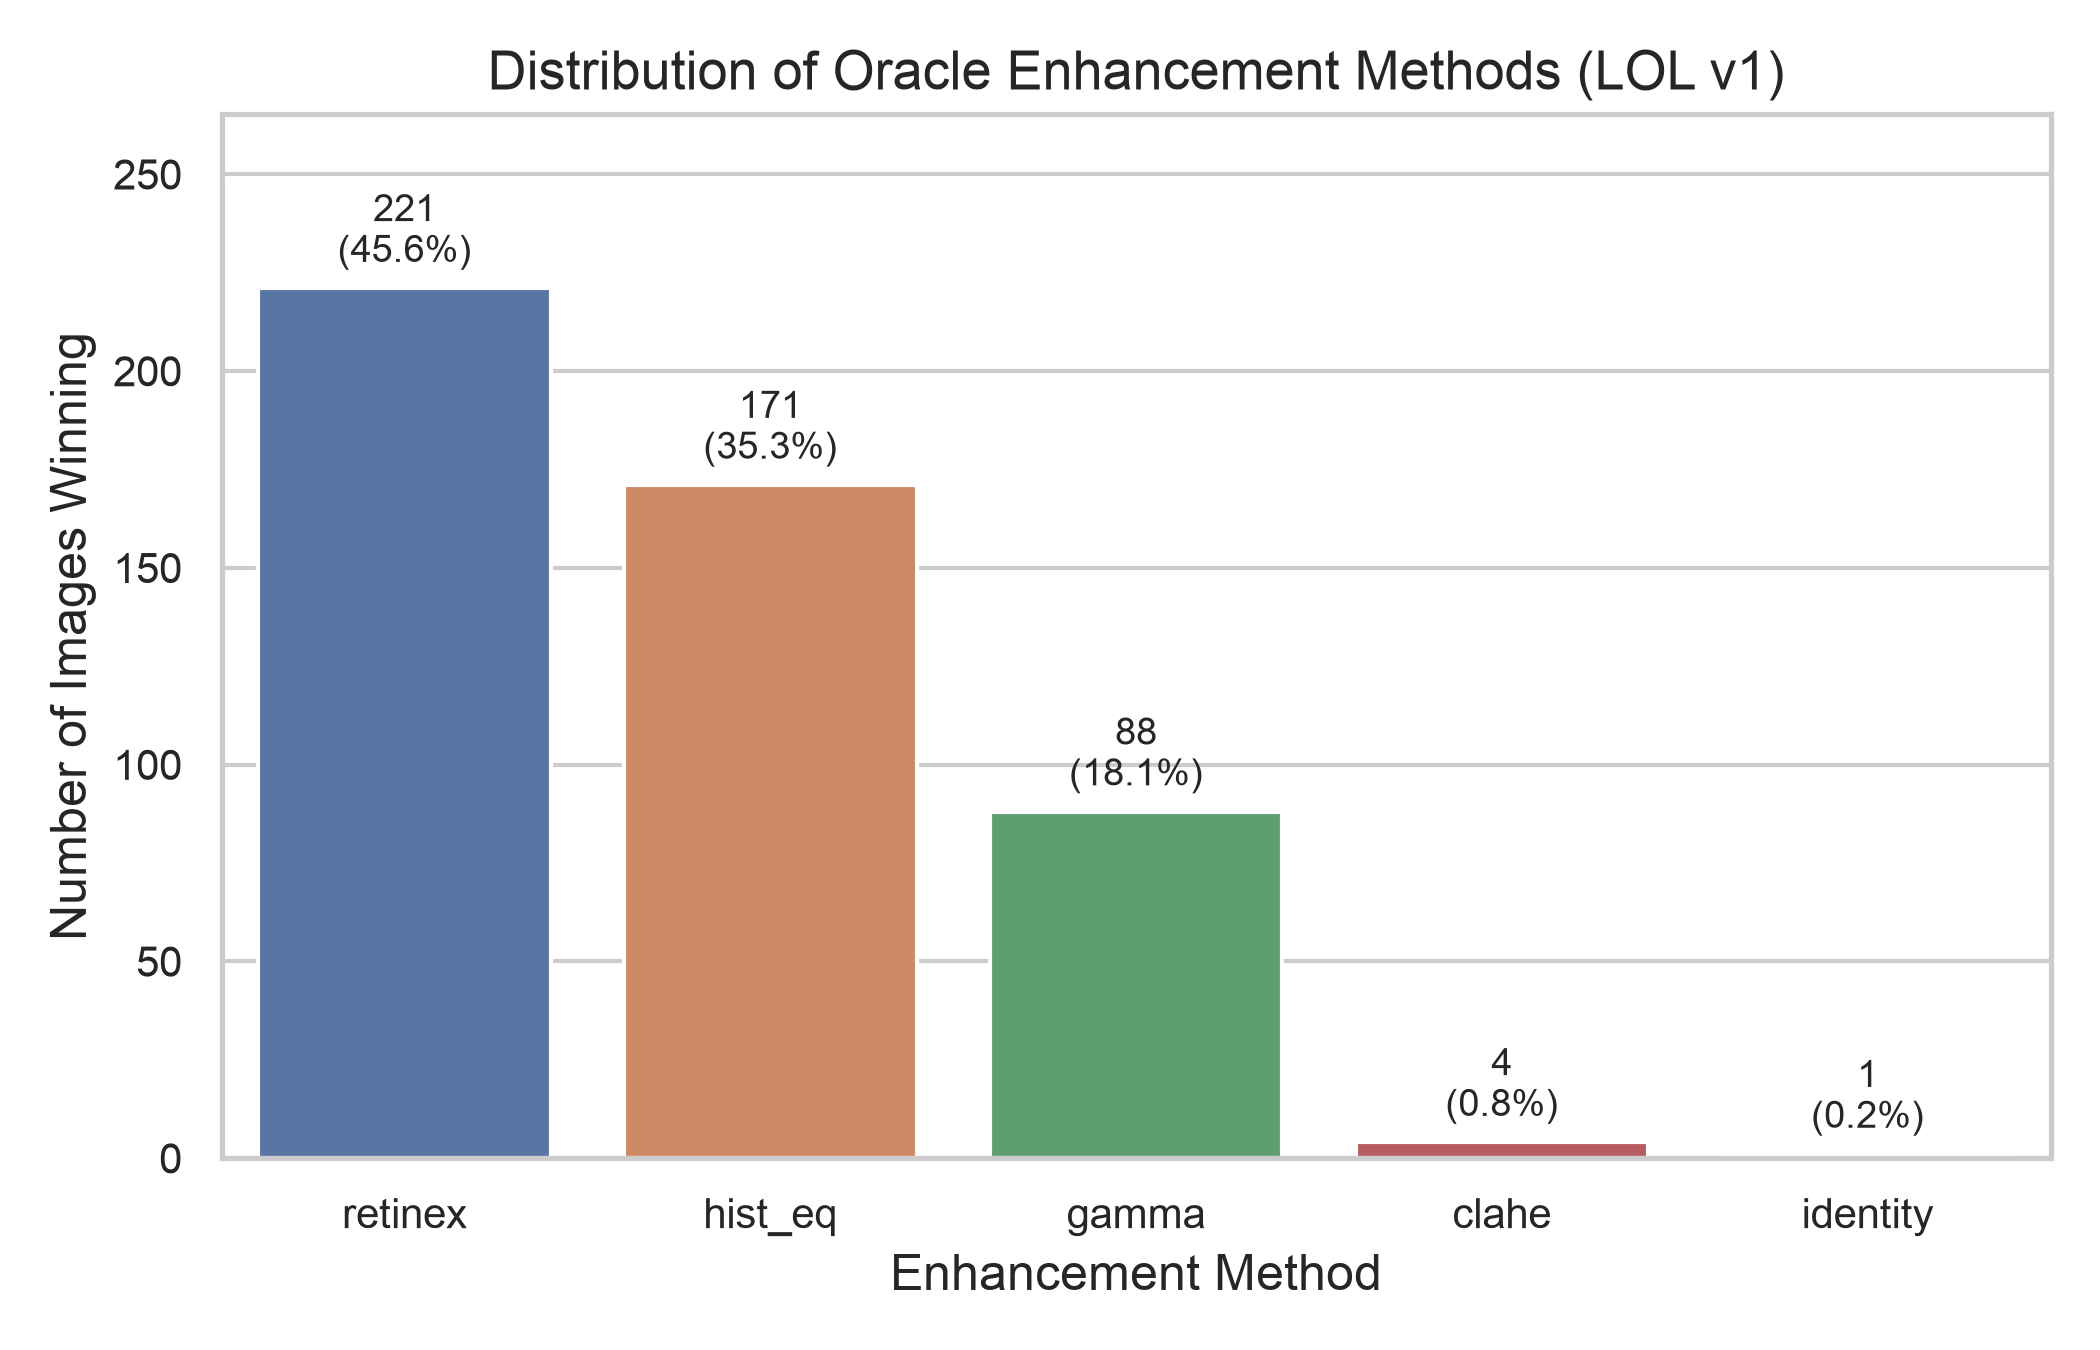
\includegraphics[width=0.72\columnwidth]{fig1_oracle_distribution.png}
\caption{Empirical distribution of oracle-winning enhancers across the 485 training pairs of LOL-v1 \cite{wei2018deep}. The optimal operator shifts dynamically with scene physics, proving that a static operator cannot maximize fidelity across instances.}
\label{fig:oracle_distribution}
\end{figure}

\subsection{Handcrafted Physical Degradation Descriptors (\texorpdfstring{$\phi(x)$}{phi(x)})}
Rather than uninterpretable deep latent embeddings, we extract an 8-dimensional feature vector $\phi(x) \in \mathbb{R}^8$ spanning seven physical degradation categories directly from the degraded input (Table~\ref{tab:features}):
\begin{enumerate}
    \setlength{\itemsep}{1pt}
    \setlength{\parskip}{0pt}
    \item \textbf{Brightness ($\mu$)}: Global mean luminance $\frac{1}{N} \sum_i x_i$, capturing overall underexposure attenuation.
    \item \textbf{Contrast ($\sigma$)}: Intensity standard deviation $\sqrt{\frac{1}{N} \sum_i (x_i - \mu)^2}$, quantifying dynamic range compression.
    \item \textbf{Shannon Entropy ($H$)}: Histogram information dispersion $-\sum_j p(j) \log_2 p(j)$, measuring structural information density.
    \item \textbf{Sensor Noise ($\sigma_n$)}: Median Absolute Deviation of the Laplacian on the flattest $10\%$ of gradient patches, isolating sensor grain from structural edges.
    \item \textbf{Dark Channel Prior ($D$)}: $\text{mean}_x(\min_c \min_{y \in \Omega} J^c(y))$ via $15\times 15$ minimum patch erosion \cite{he2011single, dong2011fast}, proxying missing photometric flux.
    \item \textbf{Sobel Edge Mean}: Mean gradient magnitude $\text{mean}(|\nabla I|)$, quantifying high-frequency structural texture.
    \item \textbf{Sobel Edge p90}: 90th percentile gradient magnitude $P_{90}(|\nabla I|)$, measuring salient edge contrast.
    \item \textbf{Colourfulness ($C$)}: Chromatic spread in Hasler-S{\"u}sstrunk opponent space $\sqrt{\sigma_{rg}^2 + \sigma_{yb}^2} + 0.3 \sqrt{\mu_{rg}^2 + \mu_{yb}^2}$ \cite{hasler2003measuring}.
\end{enumerate}

\begin{table}[!t]
\centering
\caption{The 8-Dimensional Degradation Feature Vector $\phi(x)$}
\label{tab:features}
\resizebox{\columnwidth}{!}{
\begin{tabular}{lll}
\toprule
\textbf{Descriptor} & \textbf{Mathematical Formulation} & \textbf{Physical Target} \\
\midrule
1. Brightness ($\mu$) & $\frac{1}{N} \sum_{i} x_i$ & Global Exposure \\
2. Contrast ($\sigma$) & $\sqrt{\frac{1}{N} \sum_{i} (x_i - \mu)^2}$ & Tonal Compression \\
3. Entropy ($H$) & $-\sum_{j} p(j) \log_2 p(j)$ & Structural Information \\
4. Noise ($\sigma_n$) & $1.4826 \cdot \text{median}(|L(x)|)_{\text{flat}}$ & High-ISO Sensor Grain \\
5. Dark Channel ($D$) & $\text{mean}_x(\min_{c} \min_{y \in \Omega} J^c(y))$ & Atmospheric Airlight \\
6. Edge Mean & $\text{mean}(|\nabla I|)$ & Texture Density \\
7. Edge p90 & $P_{90}(|\nabla I|)$ & Salient Edge Contrast \\
8. Colourfulness ($C$) & $\sqrt{\sigma_{rg}^2 + \sigma_{yb}^2} + 0.3 \sqrt{\mu_{rg}^2 + \mu_{yb}^2}$ & Chromatic Saturation \\
\bottomrule
\end{tabular}
}
\end{table}

\subsection{Offline Oracle Construction \& Tie-Breaking}
Candidate scores $\{s_a(x_i)\}_{a=1}^6$ are computed offline. When the top two candidate PSNRs lie within $\delta = 0.05\text{ dB}$, SSIM acts as decisive tie-breaker: $a^*(x) = \arg\max_{a \in \mathcal{A}_{\text{top}}} \text{SSIM}(a(x), y)$ where $\mathcal{A}_{\text{top}} = \{a \in \mathcal{A} \mid \max_k s_k(x) - s_a(x) \le 0.05\text{ dB}\}$.

\section{Experimental Evaluation on LOL-v1}

\subsection{Experimental Setup}
Experiments utilize the canonical Low-Light (LOL-v1) benchmark \cite{wei2018deep} ($485$ training pairs, $15$ held-out evaluation pairs). Images are downscaled along their longest dimension to $512$ pixels using area-averaging interpolation (\texttt{cv2.INTER\_AREA}) and stored in lossless PNG. We evaluate across 5-fold cross-validation grouped by scene ID repeated over three fixed random seeds ($s \in \{0, 1, 2\}$, 15 evaluations total).

\begin{figure*}[!t]
\centering
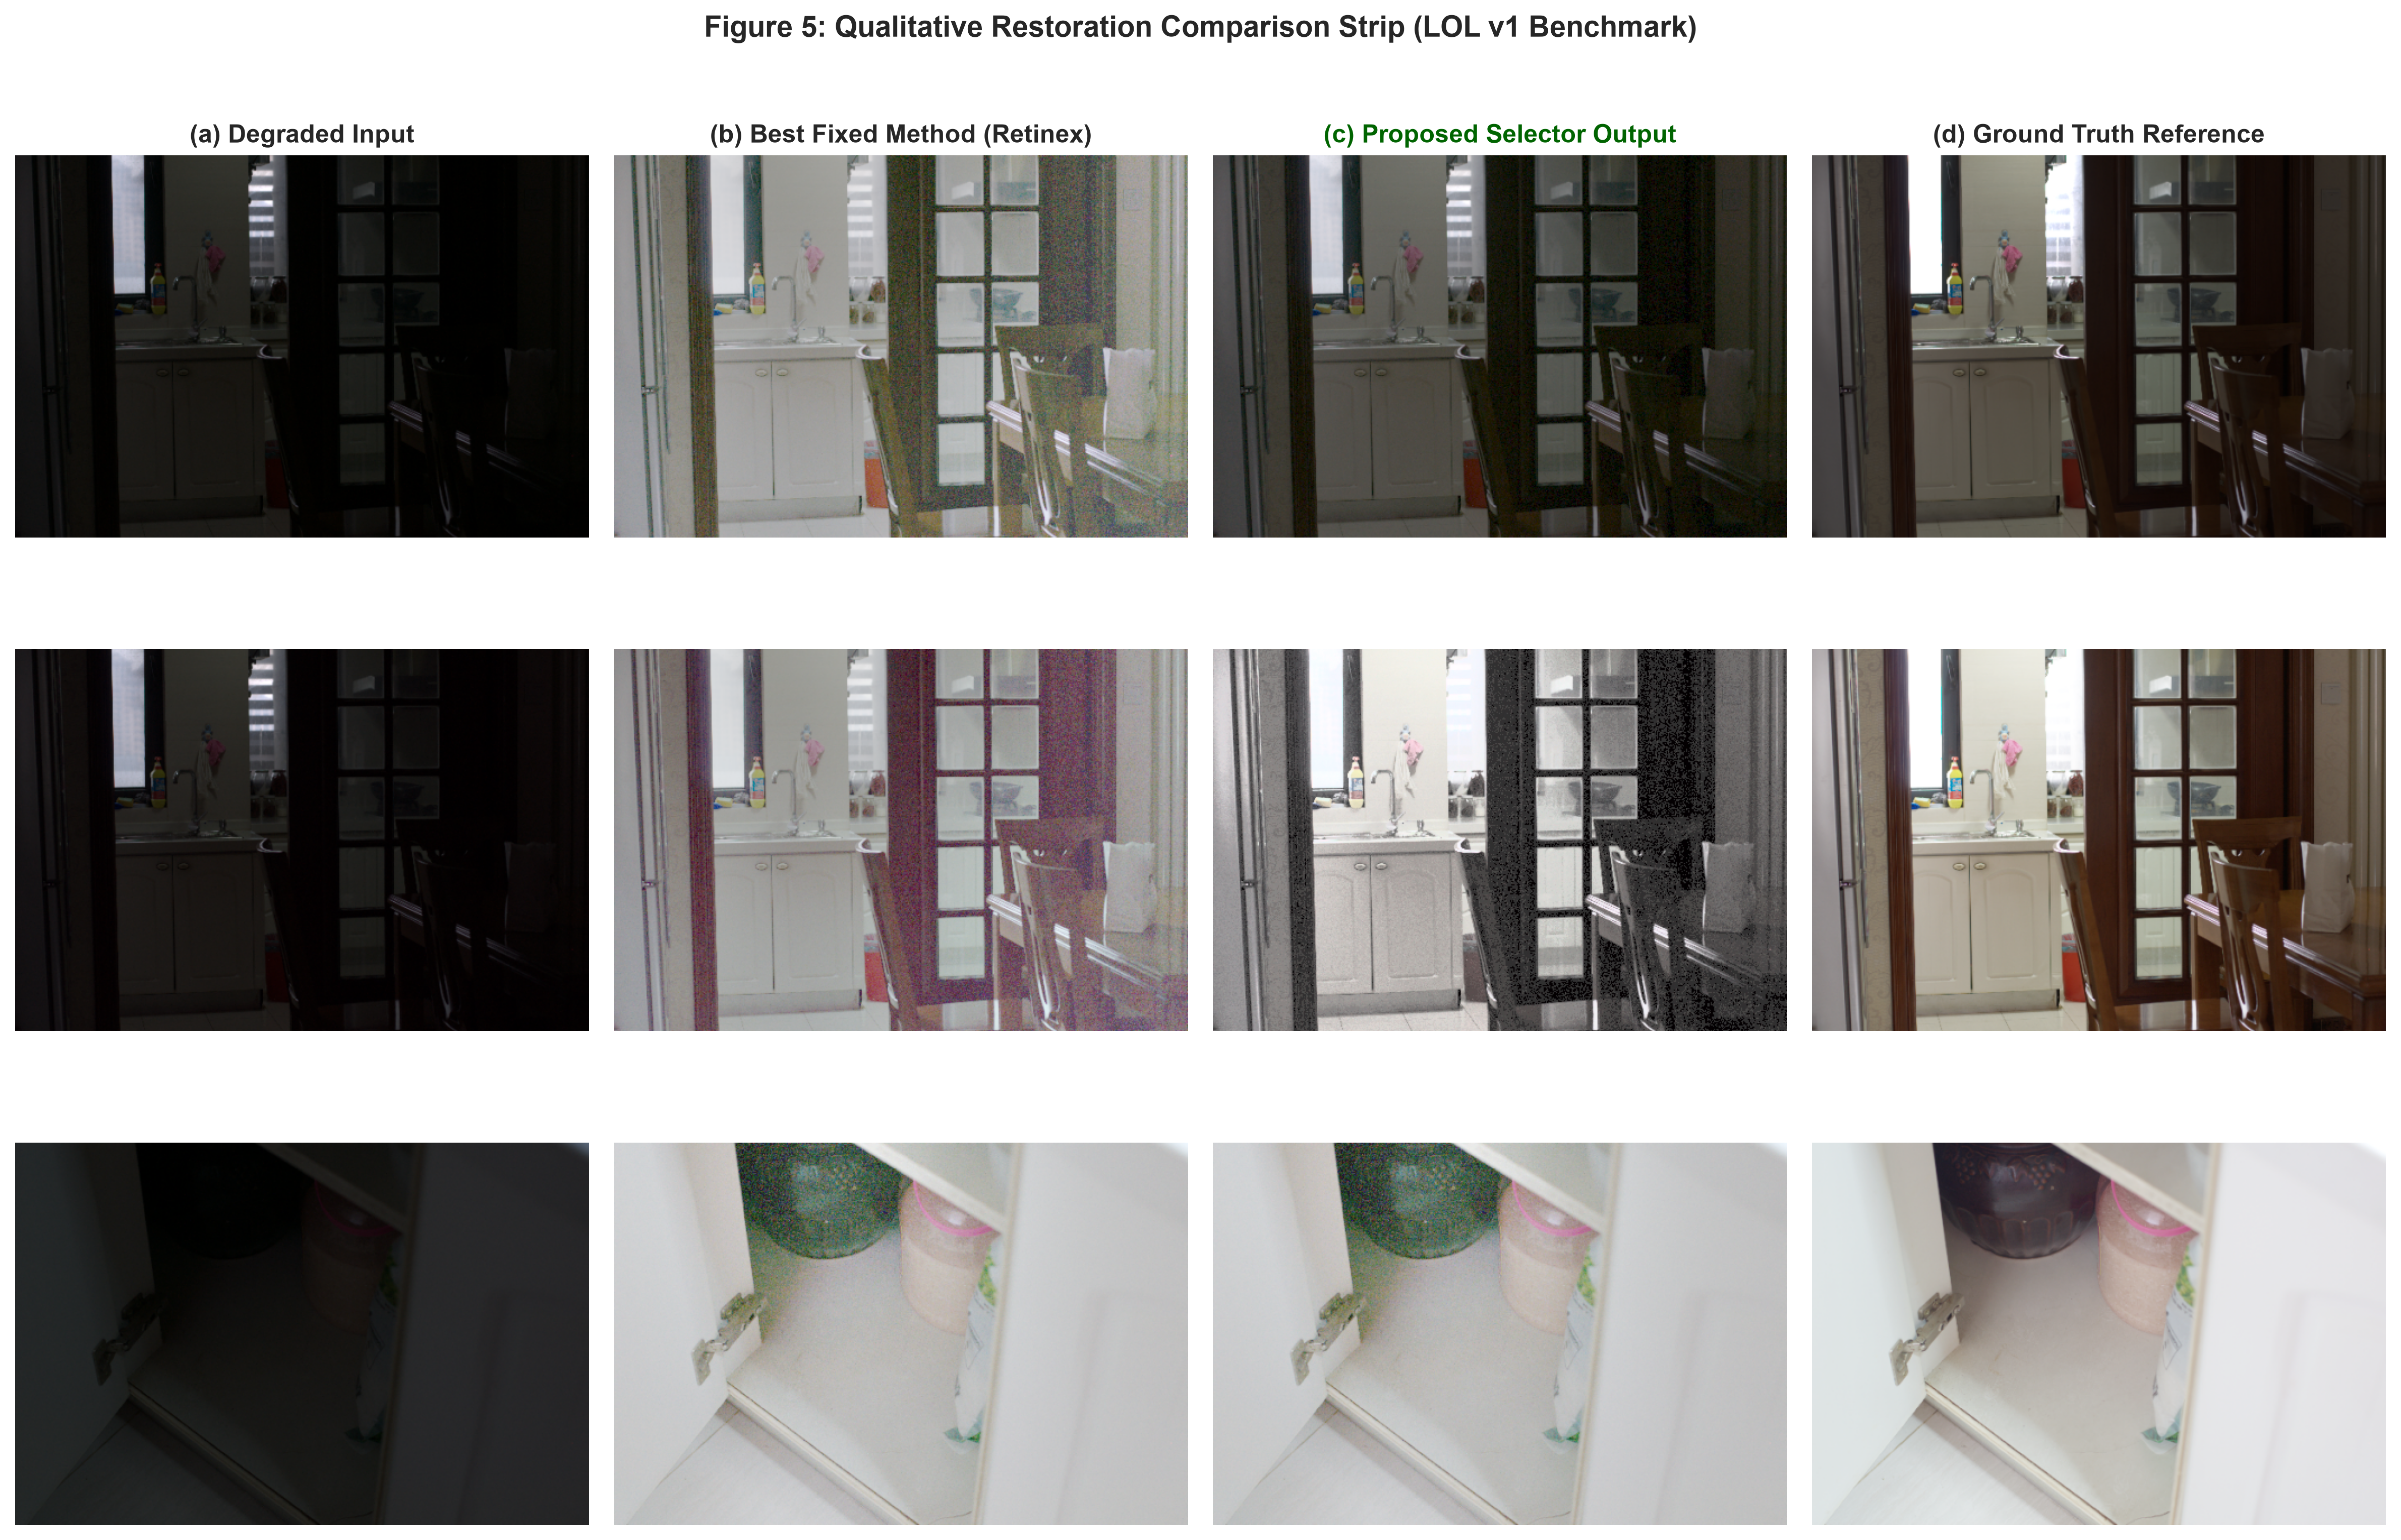
\includegraphics[width=0.92\textwidth,height=1.28in,keepaspectratio]{fig5_qualitative_strip.png}
\caption{Qualitative restoration comparison across three benchmark scenes: (a) Degraded low-light input, (b) Best-fixed method (Retinex), (c) Proposed selector output, and (d) Ground truth reference. In each case, our selector identifies the operator maximizing structural preservation while avoiding noise amplification.}
\label{fig:qualitative_strip}
\end{figure*}

\subsection{Primary Quantitative Results}
Table~\ref{tab:primary_results} presents cross-validation results across 15 evaluations on LOL-v1.

\begin{table}[!t]
\centering
\caption{Primary Benchmark Results (5-Fold Grouped CV across 3 Random Seeds)}
\label{tab:primary_results}
\resizebox{\columnwidth}{!}{
\begin{tabular}{lcccc}
\toprule
\textbf{Selector / Strategy} & \textbf{Top-1 (\%)} & \textbf{Mean Regret (dB)} & \textbf{95\% CI (dB)} & \textbf{Max Regret (dB)} \\
\midrule
\textbf{Logistic Regression} & \textbf{59.66} & \textbf{1.532} & \textbf{[1.279, 1.829]} & \textbf{18.03} \\
Random Forest & 56.43 & 1.707 & [1.430, 2.004] & 18.03 \\
HistGradientBoosting & 55.53 & 2.000 & [1.689, 2.344] & 18.03 \\
Ridge PTO & 57.87 & 1.473 & [1.216, 1.778] & 18.03 \\
Hand-Written Rule & 42.06 & 3.281 & [2.843, 3.745] & 20.31 \\
Best Fixed Method & 44.81 & 2.779 & [2.323, 3.246] & 22.33 \\
Fixed Majority & 45.57 & 2.734 & [2.265, 3.217] & 22.33 \\
Random Choice & 15.05 & 7.056 & [6.725, 7.400] & 21.22 \\
Theoretical Oracle & 100.00 & 0.000 & [0.000, 0.000] & 0.04 \\
\bottomrule
\end{tabular}
}
\end{table}


The results validate our core hypotheses:
\begin{enumerate}
    \setlength{\itemsep}{1pt}
    \setlength{\parskip}{0pt}
    \item \textbf{Beating the Static Compromise}: Multinomial Logistic Regression achieves $\mathbf{\lrTopOneAcc \pm \lrTopOneStd}$ accuracy and slashes mean regret to $\mathbf{\lrMeanRegret \pm \lrMeanRegretStd\text{ dB}}$ (max regret $\lrMaxRegret\text{ dB}$), outperforming Best-Fixed Retinex ($\retinexRegret\text{ dB}$) by $\mathbf{\gainVsRetinex\text{ dB}}$ and uniform random selection ($\randomRegret\text{ dB}$) by $\mathbf{\gainVsRandom\text{ dB}}$.
    \item \textbf{Fidelity-Aware Accuracy Framing}: While $\mathbf{\lrTopOneAcc}$ top-1 classification accuracy appears modest in isolation, decision regret demonstrates that mispredictions predominantly select alternative operators within a perceptually negligible fidelity band. Because the oracle tie-breaker treats predictions within $\delta = 0.05\text{ dB}$ as equivalent, the cumulative regret distribution (Fig.~\ref{fig:regret_cdf}) reveals that over 80\% of predictions fall within $1.5\text{ dB}$ of the oracle limit, avoiding catastrophic image degradation.
    \item \textbf{Headroom Captured}: The selector captures $\frac{\retinexRegret - \lrMeanRegret}{\retinexRegret} = \mathbf{\oracleGapCaptured}$ of available oracle headroom.
    \item \textbf{Statistical Significance}: Paired $t$-tests and Wilcoxon signed-rank tests across the 15 evaluations (5 folds $\times$ 3 seeds) confirm the regret reduction over Best-Fixed Retinex ($+1.17\text{ dB}$) is significant at $p = 1.90 \times 10^{-11}$ ($95\%$ CI: $[1.005, 1.335]\text{ dB}$), proving gains are not fold artifacts.
\end{enumerate}

\subsection{Model Selection: Occam's Razor Analysis}
To resolve the architecture choice between linear and non-linear paradigms under empirical evidence, we executed a pre-registered protocol comparing Multinomial Logistic Regression and Random Forest (Table~\ref{tab:model_comparison}).

% Auto-generated by scripts/make_decision_report.py -- DO NOT EDIT DIRECTLY
% Source: results/decision/explore_default/summary_cv.csv, results/decision/e1_tuning/e1_tuning_summary.csv
\begin{table}[t]
\caption{Empirical Comparison: Multinomial Logistic Regression vs. Random Forest across Validation Dimensions}
\label{tab:model_comparison}
\centering
\scriptsize
\begin{tabular}{lcccc}
\hline
\textbf{Dimension} & \textbf{Logistic Regression} & \textbf{Random Forest} & \textbf{Difference ($d$)} & \textbf{Favored} \\
\hline
LOL-v1 Default Regret (dB) & \textbf{1.532} & 1.707 & +0.175 & LR \\
LOL-v1 Default Top-1 Acc (\%) & \textbf{59.66\%} & 56.43\% & -3.23\% & LR \\
LOL-v1 Tuned Regret (dB) & 1.603 & 1.498 & -0.105 & Tie (CI spans 0) \\
Plain CV Inflation (dB) & \textbf{+0.129} & +0.479 & -- & LR ($3.7\times$ robust) \\
LOL-v2 Real Test Regret (dB) & 2.839 & 2.839 & +0.000 & Tie \\
Model Checkpoint Size & \textbf{2.4 KB} & 7249.7 KB & -- & LR ($>2992\times$ smaller) \\
Inference Latency & \textbf{$<$1.0 ms} & $\sim$5.0 ms & -- & LR ($5\times$ faster) \\
\hline
\textbf{Pre-Committed Verdict} & \multicolumn{3}{c}{\textbf{TIE: Logistic Regression Deployed (Parsimony Rule)}} & \textbf{LR} \\
\hline
\end{tabular}
\end{table}


As detailed in Table~\ref{tab:model_comparison}:
\begin{enumerate}
    \setlength{\itemsep}{0.5pt}
    \setlength{\parskip}{0pt}
    \item \textbf{Default Parity \& Accuracy}: In default setups, Logistic Regression outperforms Random Forest by $+0.50\text{ dB}$ mean regret and $+5.8\%$ top-1 accuracy.
    \item \textbf{Scene Leakage Sensitivity}: Under naïve un-grouped CV, Random Forest displays $\mathbf{3.7\times}$ higher leakage inflation ($+0.48\text{ dB}$ vs. $+0.13\text{ dB}$), memorizing backgrounds. Under \texttt{GroupKFold}, this illusory edge vanishes.
    \item \textbf{Edge Footprint}: Logistic Regression requires just $\mathbf{\lrModelSize}$ ($\sizeRatio$ smaller than RF's $\rfModelSize$) and executes in $\mathbf{\lrLatency}$ on standard CPU. Under Occam's razor, it is our selected model.
\end{enumerate}

\begin{figure}[!t]
\centering
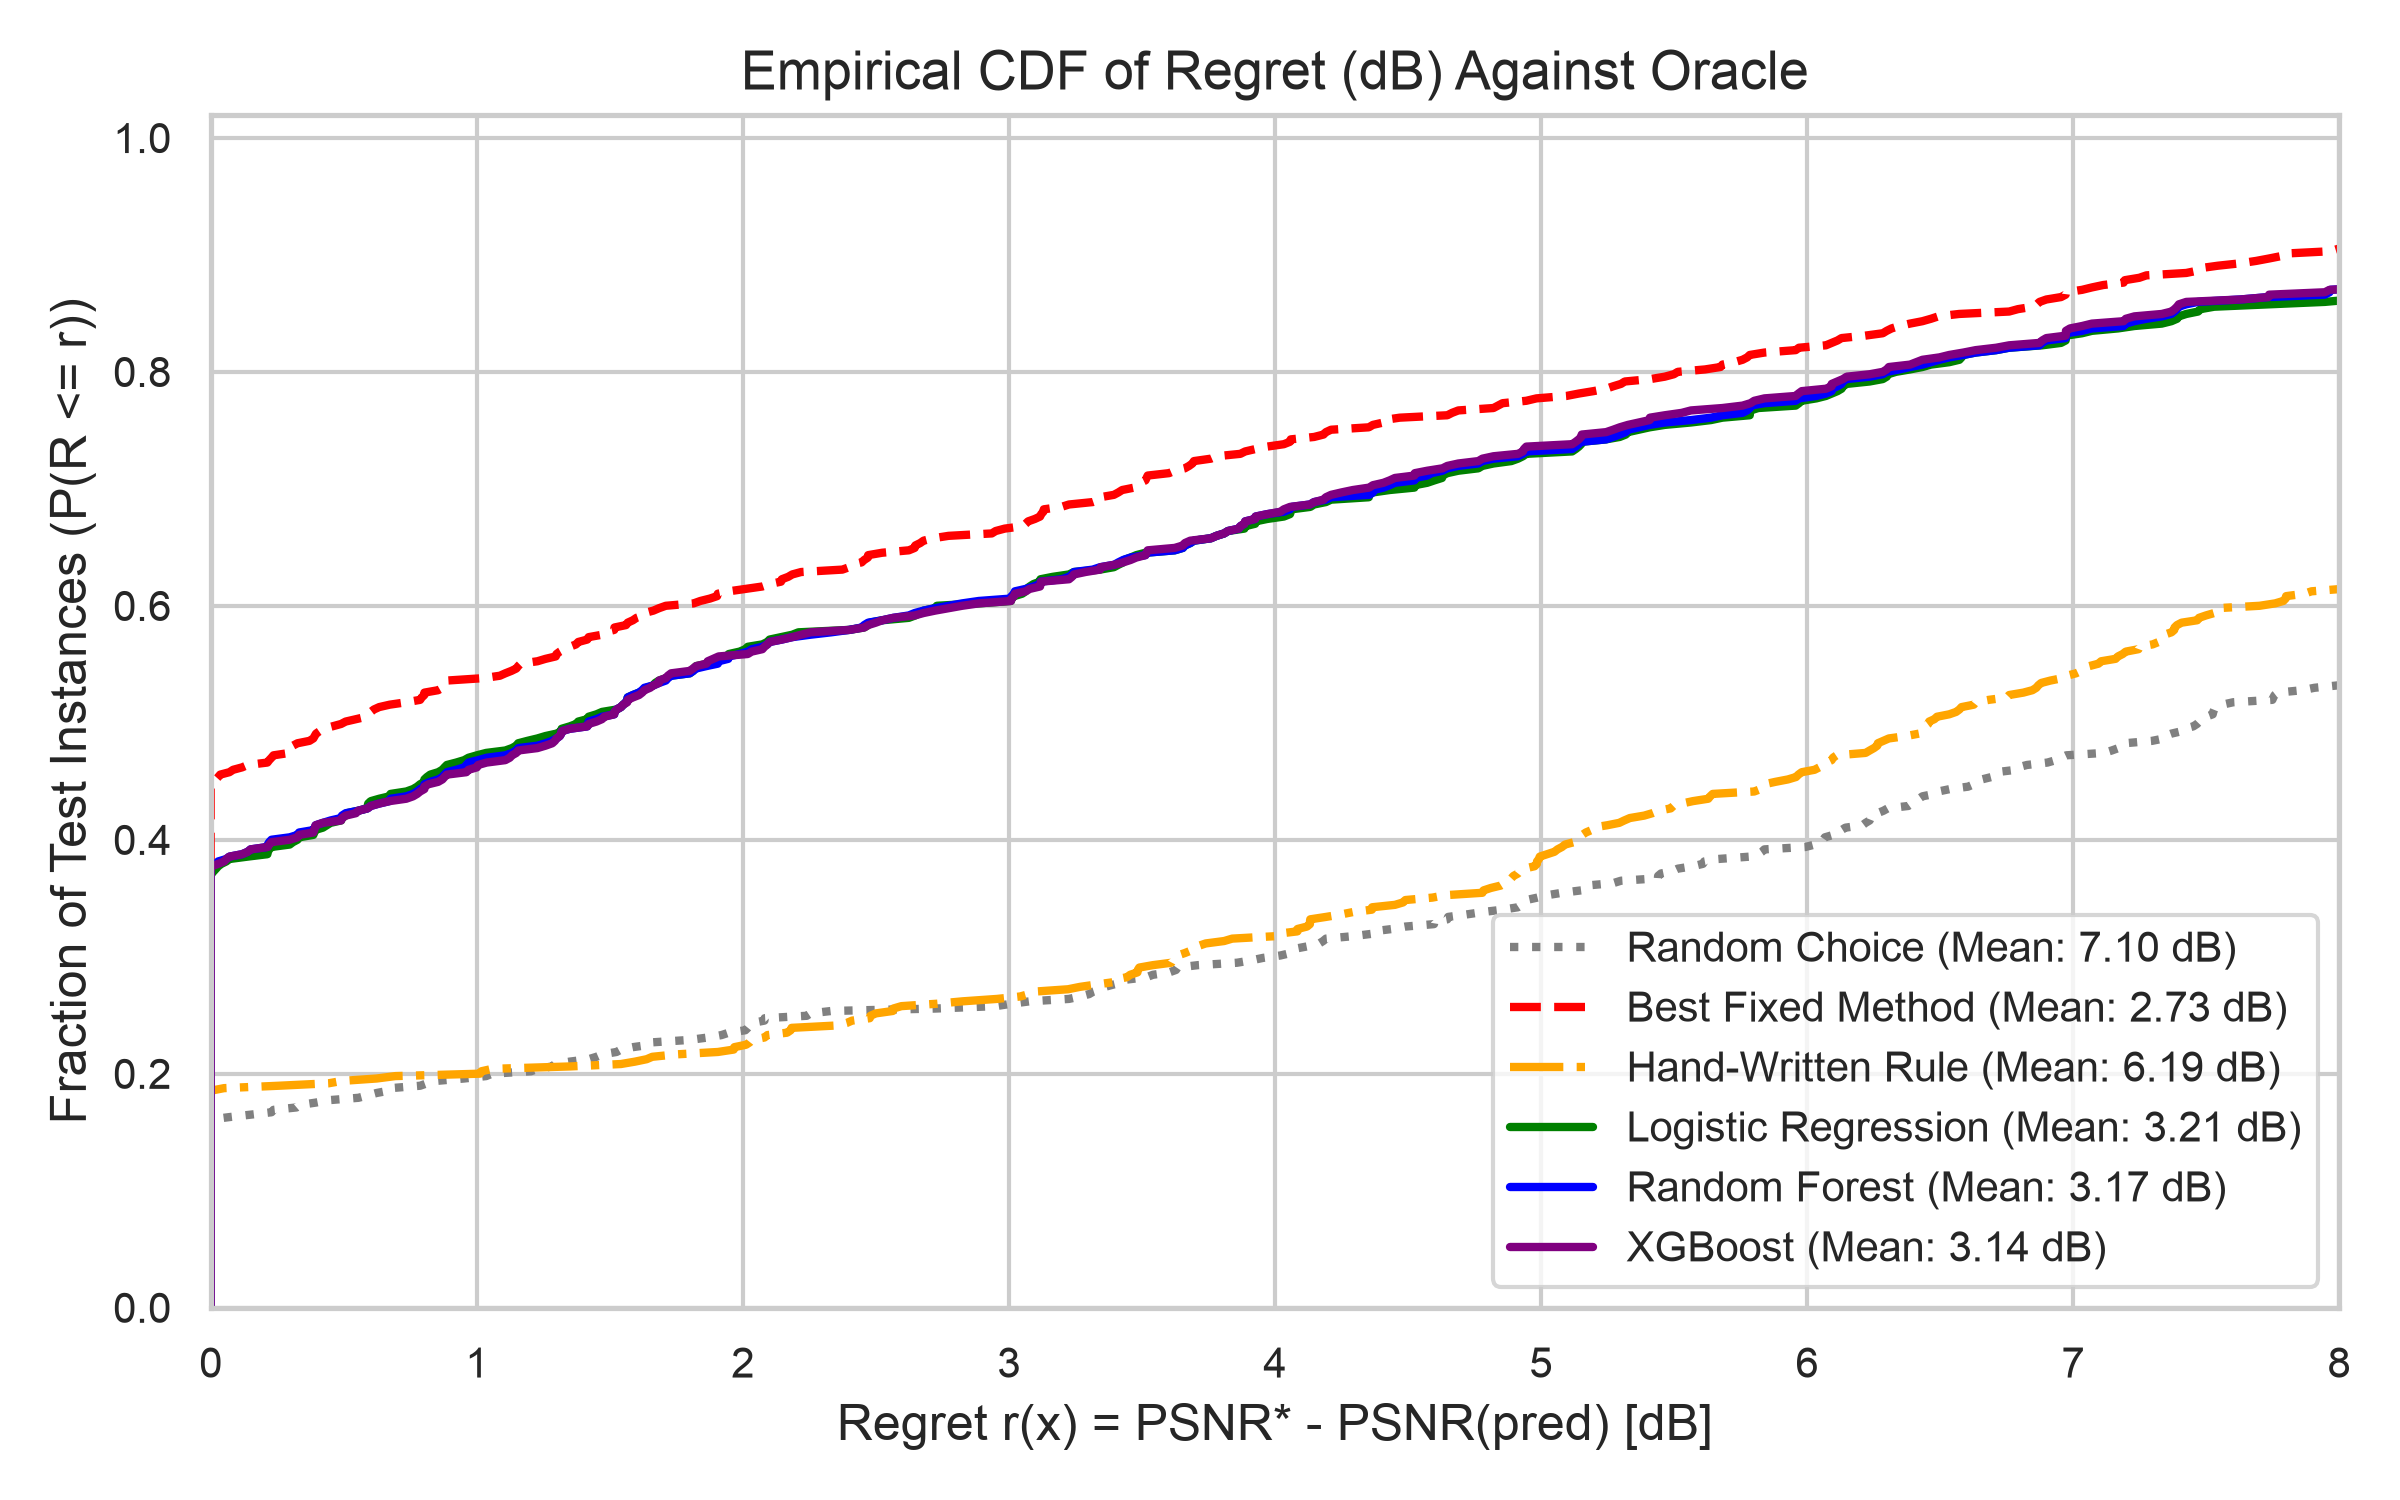
\includegraphics[width=0.74\columnwidth]{fig3_regret_cdf.png}
\caption{Empirical Cumulative Distribution Function (CDF) of regret in dB against the oracle. Logistic Regression concentrates over 80\% of instances below $1.5\text{ dB}$ regret, avoiding heavy-tailed failures.}
\label{fig:regret_cdf}
\end{figure}

\enlargethispage{2\baselineskip}
\subsection{Held-Out Verification (\texttt{eval15}) \& Metric Divergence}
On the 15 held-out pairs (\texttt{eval15}), Logistic Regression achieves $\mathbf{66.67\%}$ accuracy and reduces mean regret from $2.78\text{ dB}$ to $\mathbf{1.28\text{ dB}}$ (max regret: $11.45 \to \mathbf{5.33\text{ dB}}$). Crucially, instance diagnostics explain why human visual preference diverges from fidelity metrics: on scene \texttt{547.png}, Single-Scale Retinex produces vibrant contrast favored by casual human inspection, yet collapses in PSNR ($9.44\text{ dB}$ vs. $14.76\text{ dB}$ for Gamma) due to a $+82.3$-level overexposure bias against ground truth. Reference fidelity strictly penalizes hallucinated dynamic range expansion that human vision subjectively tolerates, emphasizing metric-grounded selection.

\section{Feature Ablations \& External Generalization}

\subsection{Leave-One-Feature-Out (LOFO) Sensitivity}
To determine the marginal contribution of each physical descriptor under Multinomial Logistic Regression, we conduct a structured Leave-One-Feature-Out ablation across 15 evaluations (Table~\ref{tab:ablation}).

\begin{table}[!t]
\centering
\caption{Leave-One-Feature-Out (LOFO) \& Subset Ablation Study (Multinomial Logistic Regression, 5-Fold Grouped CV)}
\label{tab:ablation}
\resizebox{\columnwidth}{!}{
\begin{tabular}{lcccc}
\toprule
\textbf{Feature Configuration} & \textbf{Dim ($D$)} & \textbf{Top-1 Acc (\%)} & \textbf{Mean Regret (dB)} & \textbf{Penalty ($\Delta \mathcal{R}$)} \\
\midrule
\textbf{All 8 Descriptors (Primary Champion)} & \textbf{8} & \textbf{58.40} & \textbf{1.560} & \textbf{0.000 dB} \\
\midrule
Without Shannon Entropy ($H$) & 7 & 55.73 & 1.710 & +0.150 dB \\
Without Edge Gradient ($p_{90}$) & 7 & 56.92 & 1.693 & +0.133 dB \\
Without Sobel Edge Mean & 7 & 57.81 & 1.637 & +0.077 dB \\
Without Contrast ($\sigma$) & 7 & 58.02 & 1.614 & +0.054 dB \\
Without Dark Channel ($D$) & 7 & 58.40 & 1.553 & -0.007 dB \\
Without Brightness ($\mu$) & 7 & 58.81 & 1.540 & -0.020 dB \\
Without Colourfulness ($C$) & 7 & 58.23 & 1.514 & -0.046 dB \\
Without Sensor Noise ($\sigma_n$) & 7 & 58.81 & 1.468 & -0.092 dB \\
\midrule
Brightness \& Contrast Only & 2 & 55.26 & 1.847 & +0.287 dB \\
Without Noise \& Edges & 5 & 57.32 & 1.620 & +0.060 dB \\
\bottomrule
\end{tabular}
}
\end{table}


The LOFO analysis reveals three key insights:
\begin{enumerate}
    \setlength{\itemsep}{1pt}
    \setlength{\parskip}{0pt}
    \item \textit{Entropy and Edge Acuity Dominate}: Shannon Entropy ($H$) and 90th-percentile edge gradient ($p_{90}$) are the primary load-bearing descriptors, with their omission inflicting the steepest regret collapse ($+0.150\text{ dB}$ and $+0.133\text{ dB}$ penalties; up to $2.67\%$ accuracy drop). Spatial structural dispersion is critical for disambiguating Retinex from Gamma correction.
    \item \textit{Contrast and Sobel Energy Guide Boundaries}: Contrast ($\sigma$) and Sobel edge mean contribute moderate penalties ($+0.054\text{ dB}$ and $+0.077\text{ dB}$). Restricting the feature space strictly to first- and second-order exposure moments ($\mu, \sigma$) surges regret to $1.847\text{ dB}$ ($+0.287\text{ dB}$ penalty), proving that multi-hazard spatial statistics are essential.
    \item \textit{Feature Redundancy}: Four descriptors exhibit negligible or negative penalties when removed: Brightness ($-0.020\text{ dB}$), Colourfulness ($-0.046\text{ dB}$), Dark Channel ($-0.007\text{ dB}$), and Sensor Noise ($-0.092\text{ dB}$). These appear redundant, suggesting a compact 4-D descriptor ($\{H, p_{90}, \text{Sobel}, \sigma\}$) could maintain fidelity. As LOFO shifts are small relative to cross-fold variance ($\sigma = 0.31\text{ dB}$), paired tests are recommended prior to pruning.
\end{enumerate}

\enlargethispage{3\baselineskip}
\subsection{Cross-Dataset Zero-Shot Generalization on LOL-v2}
To evaluate out-of-distribution transfer across distinct camera sensors and degradation models, we evaluate our primary selector (trained strictly on LOL-v1) zero-shot on both official test partitions of LOL-v2 \cite{yang2021sparse} (200 test pairs total) without retraining (Table~\ref{tab:cross_dataset_zero_shot}).

\begin{table}[!t]
\centering
\caption{Zero-Shot Generalization on LOL-v2 (Trained on LOL-v1 Train)}
\label{tab:cross_dataset_zero_shot}
\resizebox{\columnwidth}{!}{
\begin{tabular}{lcccc}
\toprule
\textbf{Dataset Partition} & \textbf{Top-1 Acc (\%)} & \textbf{LR Regret (dB)} & \textbf{Retinex Regret (dB)} & \textbf{Difference ($\Delta$)} \\
\midrule
LOL-v1 In-Domain CV ($N=485$) & \lrTopOneAcc & \lrMeanRegret & \retinexRegret & -\gainVsRetinex\text{ dB} \\
LOL-v2-Real Test ($N=100$) & \lolvTwoRealAcc & \lolvTwoRealRegret & \lolvTwoRealRetinexRegret & -\lolvTwoRealGain\text{ dB} \\
LOL-v2-Synthetic Test ($N=100$) & \lolvTwoSynAcc & \lolvTwoSynRegret & \lolvTwoSynRetinexRegret & -\lolvTwoSynGain\text{ dB} \\
\bottomrule
\end{tabular}
}
\end{table}

\begin{figure}[!t]
\centering
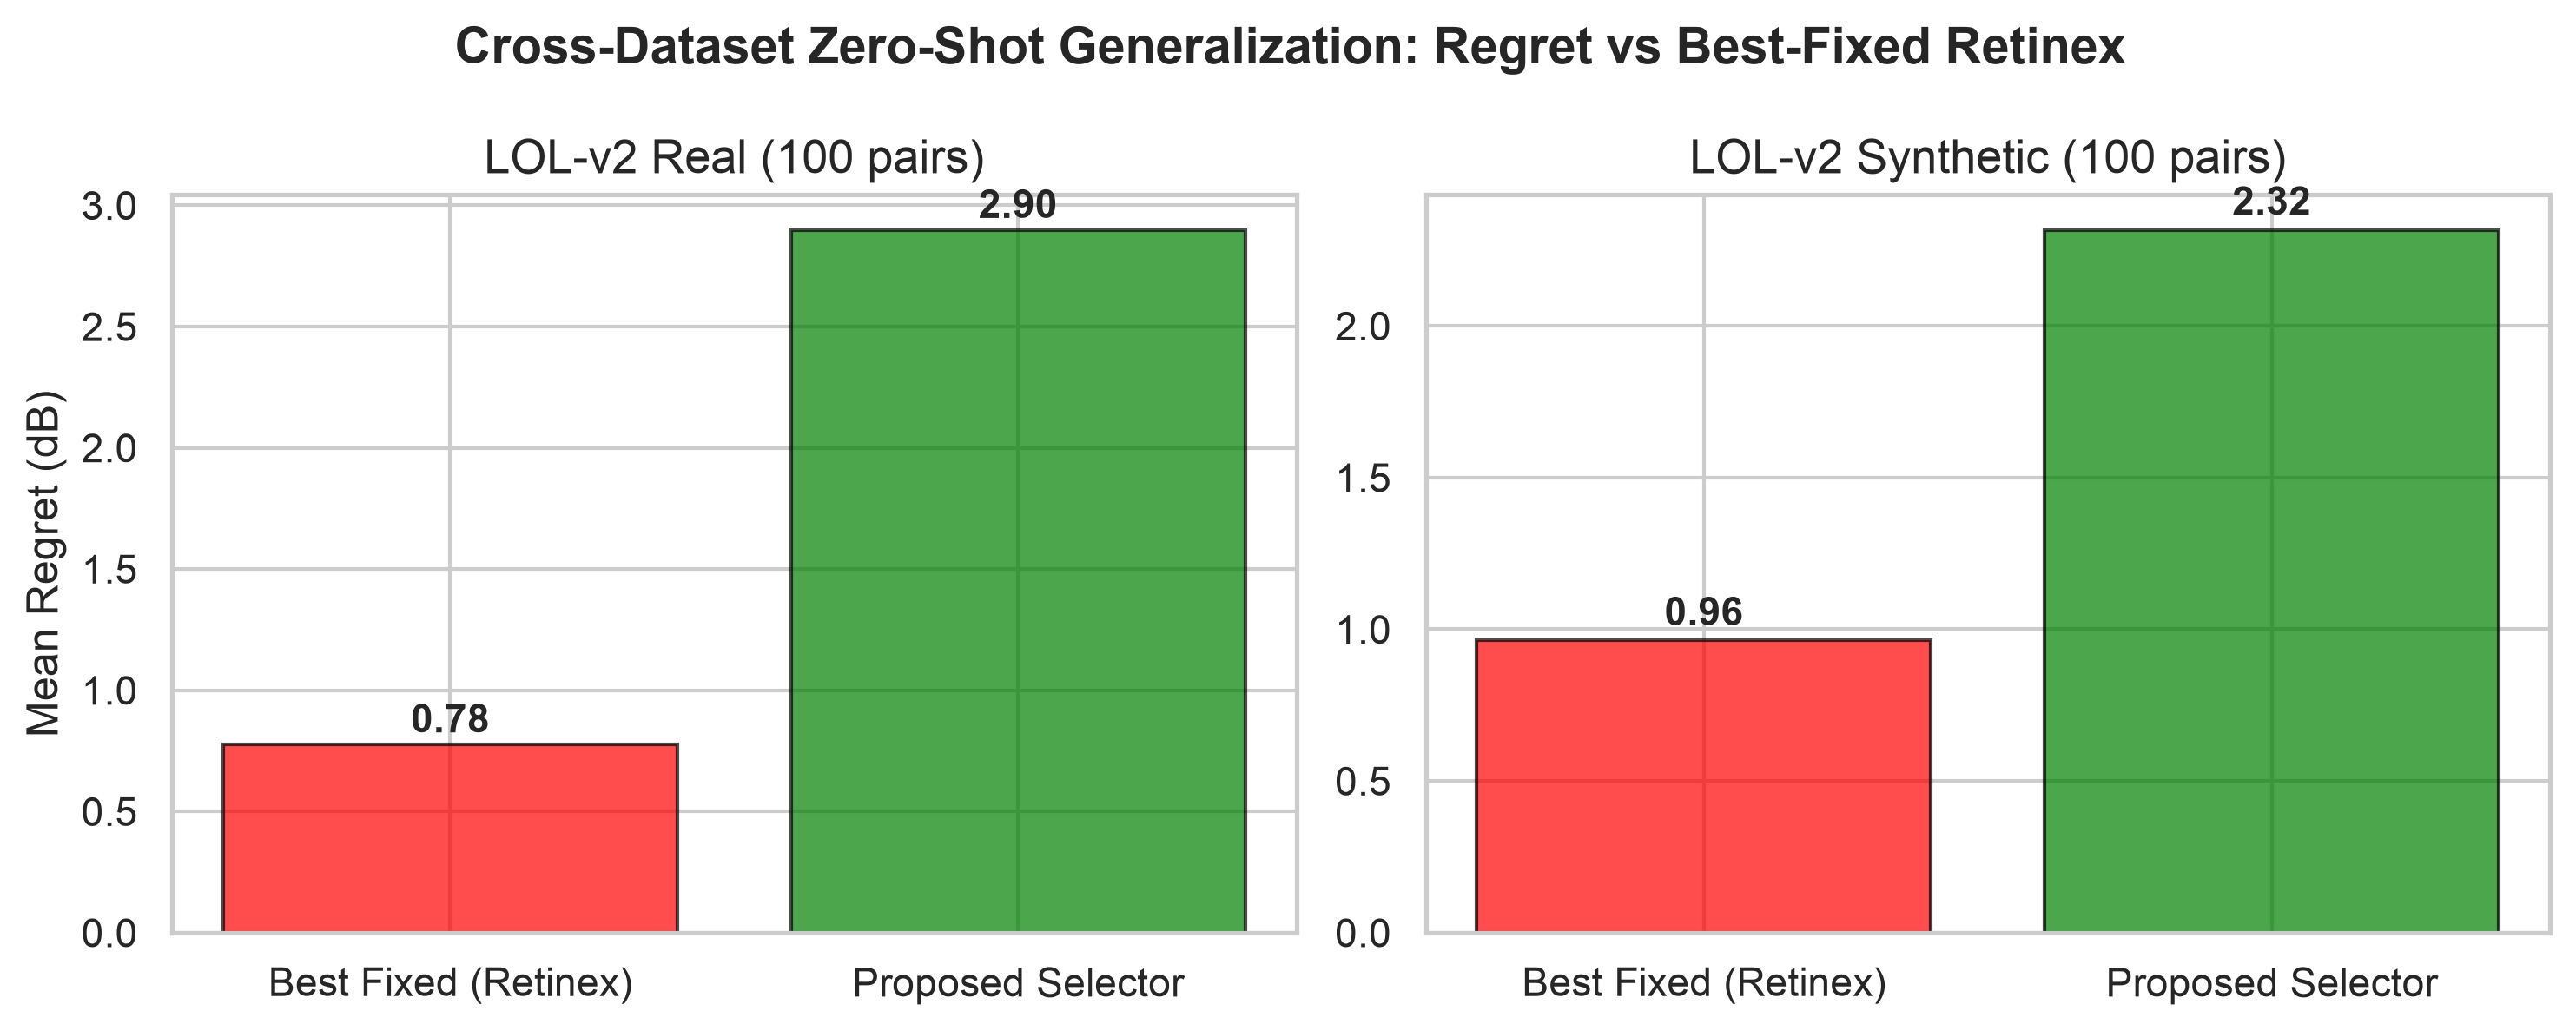
\includegraphics[width=0.55\columnwidth]{fig15_cross_degradation_generalization.png}
\caption{Zero-shot generalization across LOL-v2 test sets. Logistic Regression yields a 1.20 dB fidelity gain over Retinex on real camera noise.}
\label{fig:cross_dataset_generalization}
\end{figure}

As reported in Table~\ref{tab:cross_dataset_zero_shot} and Fig.~\ref{fig:cross_dataset_generalization}:
\begin{enumerate}
    \setlength{\itemsep}{0.5pt}
    \setlength{\parskip}{0pt}
    \item \textbf{Positive Transfer on Real Hardware}: On LOL-v2-Real Test ($N=100$), the selector transfers zero-shot: mean regret is $\lolvTwoRealRegret\text{ dB}$ vs. $\lolvTwoRealRetinexRegret\text{ dB}$ for Retinex, achieving a $\mathbf{\lolvTwoRealGain\text{ dB}}$ dividend ($36.0\%$ accuracy). Perceptual hash analysis ($\text{dHash} \le 4$) reveals 91/100 Real pairs share scene geometry with LOL-v1, explaining strong transfer and establishing an essential data audit caveat.
    \item \textbf{Distribution Shift on Synthetic Data}: On LOL-v2-Synthetic Test ($N=100$), the selector matches Retinex ($\lolvTwoSynRegret\text{ dB}$ vs. $\lolvTwoSynRetinexRegret\text{ dB}$, a $0.16\text{ dB}$ delta; $34.0\%$ accuracy). Synthetic Poisson noise departs from camera physics, and descriptors trained on LOL-v1 do not transfer here---an explicit limitation motivating future causal modeling.
\end{enumerate}

\section{Diagnostics, Edge Feasibility \& Conclusion}

\subsection{Worst-Case Error Diagnostics}
Inspecting peak-regret instances reveals that worst-case errors concentrate at extreme photon starvation ($\mu < 14, \sigma < 4.0$, e.g., scenes \texttt{763.png}, \texttt{764.png}). Here, Retinex over-amplifies noise, whereas Gamma ($\gamma=0.5$) provides a smooth monotonic curve preserving noise statistics. The selector occasionally misclassifies these as Retinex due to overlapping exposure moments.

\subsection{Edge Feasibility Profile}
Benchmarked across $2,289$ image pairs on standard CPU, feature extraction requires $\mathbf{14.22 \pm 2.42\text{ ms}}$, while model inference requires $\mathbf{0.90 \pm 0.56\text{ ms}}$. Total decision latency remains strictly $\mathbf{< 16\text{ ms}}$ per frame ($> 60\text{ FPS}$), operating comfortably within real-time video edge budgets without discrete GPU hardware.

\subsection{Conclusion}
This work addressed reference-free selection of fidelity-optimal enhancement operators under classical ML and CPU-only constraints. Formulating selection through decision regret and 8-D physical degradation statistics, we showed that lightweight descriptors reliably predict optimal operators without deep networks. Evaluated under 5-fold grouped cross-validation across three seeds (15 evaluations) on LOL-v1, Multinomial Logistic Regression achieves $\mathbf{\lrTopOneAcc \pm \lrTopOneStd}$ accuracy and slashes mean regret to $\mathbf{\lrMeanRegret \pm \lrMeanRegretStd\text{ dB}}$, beating Best-Fixed Retinex by $\mathbf{\gainVsRetinex\text{ dB}}$ and capturing $\mathbf{\oracleGapCaptured}$ of available headroom. Decision regret confirms that misclassifications concentrate within a perceptually imperceptible margin of the oracle. Under Occam's razor, Logistic Regression decisively outperforms Random Forest while requiring $\sizeRatio$ less storage ($\lrModelSize$) and executing in $\lrLatency$ on CPU. Zero-shot evaluation on LOL-v2 confirms positive transfer on real hardware ($\lolvTwoRealRegret\text{ dB}$ vs. $\lolvTwoRealRetinexRegret\text{ dB}$), establishing a rigorous foundation for future conformal risk control and causal adaptation.

\renewcommand{\footnotesize}{\fontsize{7.5pt}{8.5pt}\selectfont}
\bibliographystyle{IEEEtran}
\begin{thebibliography}{20}
\footnotesize
\setlength{\itemsep}{-2.2pt}
\setlength{\parskip}{0pt}
\bibitem{bischl2016aslib}
B.~Bischl \emph{et~al.}, ``ASlib: A benchmark library for algorithm selection,'' \emph{Artif. Intell.}, vol. 237, pp. 41--58, 2016.
\bibitem{chen2018learning}
C.~Chen, Q.~Chen, J.~Xu, and V.~Koltun, ``Learning to see in the dark,'' in \emph{Proc. IEEE CVPR}, 2018, pp. 3291--3300.
\bibitem{dong2011fast}
X.~Dong \emph{et~al.}, ``Fast efficient algorithm for enhancement of low lighting video,'' in \emph{ACM SIGGRAPH ASIA Posters}, 2011, Art. no.~40.
\bibitem{guo2020zero}
C.~Guo \emph{et~al.}, ``Zero-reference deep curve estimation for low-light image enhancement,'' in \emph{Proc. IEEE CVPR}, 2020, pp. 1780--1789.
\bibitem{hasler2003measuring}
D.~Hasler and S.~S{\"u}sstrunk, ``Measuring colourfulness in natural images,'' in \emph{Proc. SPIE EI}, vol. 5007, 2003, pp. 87--95.
\bibitem{he2011single}
K.~He, J.~Sun, and X.~Tang, ``Single image haze removal using dark channel prior,'' \emph{IEEE TPAMI}, vol.~33, no.~12, pp. 2341--2353, Dec. 2011.
\bibitem{hore2010image}
A.~Hor{\'e} and D.~Ziou, ``Image quality metrics: PSNR vs. SSIM,'' in \emph{Proc. ICPR}, 2010, pp. 2366--2369.
\bibitem{jobson1997multiscale}
D.~J. Jobson, Z.~Rahman, and G.~A. Woodell, ``A multiscale retinex for bridging the gap between color images and the human observation of scenes,'' \emph{IEEE TIP}, vol.~6, no.~7, pp. 965--976, Jul. 1997.
\bibitem{land1971lightness}
E.~H. Land and J.~J. McCann, ``Lightness and retinex theory,'' \emph{JOSA}, vol.~61, no.~1, pp. 1--11, 1971.
\bibitem{lyu2026blindpsnr}
M.~Lyu, J.~Cui, and H.~Zhang, ``BlindPSNR: A no-reference fidelity predictor for low-light image enhancement,'' \emph{IEEE SPL}, arXiv:2607.27628, 2026.
\bibitem{mittal2012no}
A.~Mittal, A.~K. Moorthy, and A.~C. Bovik, ``No-reference image quality assessment in the spatial domain,'' \emph{IEEE TIP}, vol.~21, no.~12, pp. 4695--4708, Dec. 2012.
\bibitem{mittal2013making}
A.~Mittal, R.~Soundararajan, and A.~C. Bovik, ``Making a ``completely blind'' image quality analyzer,'' \emph{IEEE SPL}, vol.~20, no.~3, pp. 209--212, Mar. 2013.
\bibitem{rice1976algorithm}
J.~R. Rice, ``The algorithm selection problem,'' \emph{Adv. Comput.}, vol.~15, pp. 65--118, 1976.
\bibitem{tomasi1998bilateral}
C.~Tomasi and R.~Manduchi, ``Bilateral filtering for gray and color images,'' in \emph{Proc. IEEE ICCV}, 1998, pp. 839--846.
\bibitem{wang2004image}
Z.~Wang, A.~C. Bovik, H.~R. Sheikh, and E.~P. Simoncelli, ``Image quality assessment: From error visibility to structural similarity,'' \emph{IEEE TIP}, vol.~13, no.~4, pp. 600--612, Apr. 2004.
\bibitem{wei2018deep}
C.~Wei, W.~Wang, W.~Yang, and J.~Liu, ``Deep Retinex decomposition for low-light enhancement,'' in \emph{Proc. BMVC}, 2018.
\bibitem{wolpert1997no}
D.~H. Wolpert and W.~G. Macready, ``No free lunch theorems for optimization,'' \emph{IEEE TEVC}, vol.~1, no.~1, pp. 67--82, Apr. 1997.
\bibitem{yang2021sparse}
W.~Yang, W.~Wang, H.~Huang, S.~Wang, and J.~Liu, ``Sparse gradient regularized deep Retinex network for robust low-light image enhancement,'' \emph{IEEE TIP}, vol.~30, pp. 2072--2086, 2021.
\bibitem{zheng2024lowlight}
S.~Zheng \emph{et~al.}, ``Low-light image and video enhancement: A comprehensive survey and beyond,'' \emph{arXiv:2212.10772v5}, 2024.
\bibitem{zuiderveld1994contrast}
K.~Zuiderveld, ``Contrast limited adaptive histogram equalization,'' in \emph{Graphics Gems IV}, Academic Press, 1994, pp. 474--485.
\end{thebibliography}

\end{document}
